\documentclass{beamer}
\usetheme{STCE}

\usepackage{beamerfoils}
\usepackage[utf8]{inputenc}
\usepackage{amsmath}
\usepackage[german]{babel} % Für deutche Umlaute
\usepackage{tabularx} % Für die TabularX Umgebung
\usepackage{listings}

\lstloadlanguages{[ISO]C++}

\lstset{basicstyle=\scriptsize}

\MyLogo{
\centering

\includegraphics[width=0.12\textwidth]{figures/logo.eps}
}

\begin{document}
\title{Korrelation und Regressionsanalyse\\
Finale Präsentation}
\author{Patrick Neidig \and Marius Grysla}
\institute{Software and Tools for Computational Engeneering}
\date{28.06.2011}
\frame{\titlepage}

\begin{frame}
 \frametitle{Inhalt}
 \tableofcontents
\end{frame}

\section{Korrelation}

\subsection{Wiederholung}
\begin{frame}
  \frametitle{Wiederholung}

\end{frame}

\subsection{Planänderungen}
\begin{frame}
  \frametitle{Planänderungen Korrelation}

\end{frame}

\section{Regression}

\subsection{Wiederholung}
\begin{frame}
  \frametitle{Wiederholung Regression}

  \begin{block}{Regression}
    Bestimmung einer Funktion die den Zusammenhang zwischen einem Regressanden und einem oder mehreren Regressoren modelliert.
  \end{block}
  
  \pause

  \begin{block}{Multipler linearer Regressionsansatz}
    \begin{equation*}
      Y_i = \beta_0 + \beta_1 x_{i1} + \dots + \beta_p x_{ip} + \epsilon_i, \quad i = 1, \dots, n
    \end{equation*}
    \begin{itemize}
    \item Anzahl der Regressoren: $p$
    \end{itemize}
  \end{block}

  \begin{itemize}
  \item Eine Transformation des Regressanden ist möglich!
  \end{itemize}

\end{frame}

\begin{frame}
  \frametitle{Berechnung Regression}

  \begin{block}{Methode der kleinsten Quadrate}
    {\centering
      $\sum\limits^{N}_{n=1} \epsilon^2_n = \epsilon^T \epsilon = (y - X \beta)^T (y - X \beta) = $
      $\Vert X\beta - y \Vert_2 \rightarrow \min\limits_{\beta}$
      \\}
  \end{block}
  
  \begin{itemize}
  \item Berechnung mittels QR-Zerlegung von $X$:
    \begin{itemize}
    \item $X = QR^*$, mit $R^* = \binom{R}{0}$
    \item $Q^T * y = \binom{c}{d}$
    \item Löse $R \hat{\beta} = c$ durch Rückwärtseinsetzen
    \end{itemize}
  \end{itemize}

  \pause

  \begin{itemize}
  \item Verfahren zur QR-Zerlegung:
    \begin{itemize}
    \item Householder Transformationen
    \item Givens Rotationen
    \item Modifiziertes Gram-Schmidt Verfahren
    \end{itemize}
  \end{itemize}

\end{frame}

\begin{frame}
  \frametitle{Ergebnis Mietdatensatz}
  
  \begin{figure}[t]
    \centering
    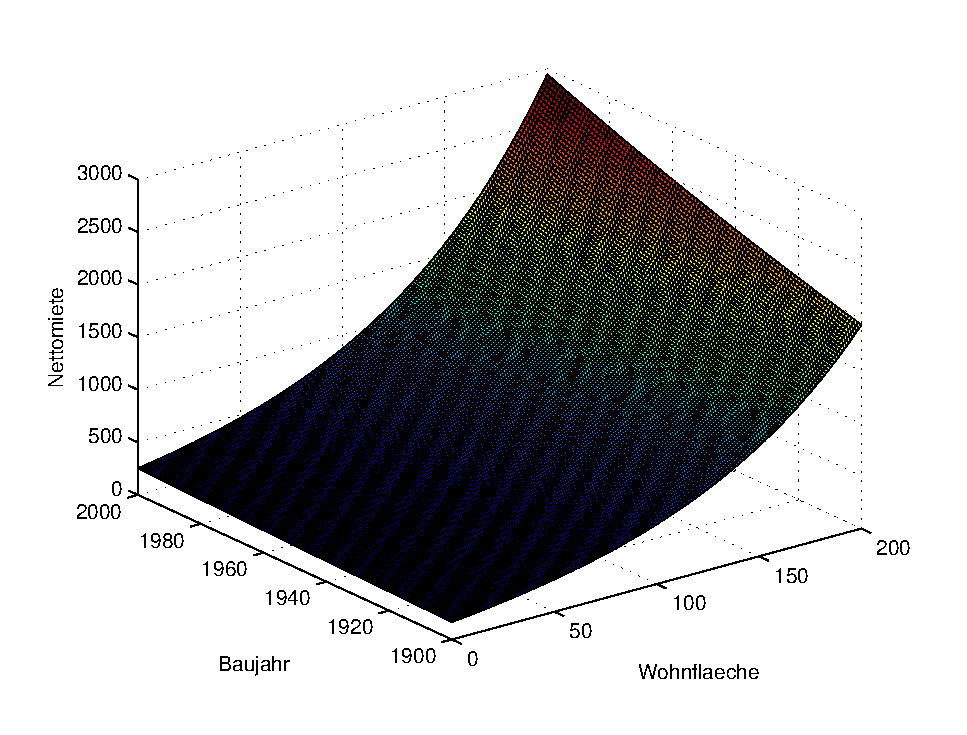
\includegraphics[width=10cm]{figures/nm_wfl_bj_log_approach.eps}
  \end{figure}

\end{frame}

\subsection{Planänderungen}
\begin{frame}
  \frametitle{Planänderungen Regression}

  \begin{itemize}
  \item Geplant:
    \begin{itemize}
    \item Einfache Regression
    \item Multiple Regression
    \item {\color<2->[gray]{0.4}Robuste Regression (optional)}
    \item Modellauswahl
    \item {\color<2->[gray]{0.4}Modellvalidierung}
    \item Leistungsanalyse
    \end{itemize}
    
    \pause\pause
  
  \item Grund: Platz!
  \end{itemize}

\end{frame}


\section{Anwendung}
\begin{frame}
  \frametitle{Testprogramm}

\end{frame}

\section{Leitungsanalyse}
\begin{frame}
  \frametitle{Leistungsanalyse}
  
  \begin{itemize}
  \item Allgemeine Informationen zur Analyse
  \item Server, 
  \end{itemize}
\end{frame}

\subsection{Gnu Scientific Library}
\begin{frame}
  \frametitle{Gnu Scientific Library}
  
  \begin{itemize}
  \item Informationen zur GSL
  \item Warum gerade diese Bibliothek?
  \end{itemize}
  
\end{frame}

\subsection{Korrelation}
\begin{frame}
  
\end{frame}

\subsection{Regression}
\begin{frame}
  \frametitle{Funktionsübersicht Regression}
  
  \begin{columns}
    \column{.45\textwidth}
    \begin{block}{GSL Funktionen}
      \alert<1>{
        gsl\_fit\_linear\\
        gsl\_fit\_wlinear\\
        gsl\_fit\_linear\_est\\
        gsl\_fit\_mul\\
        gsl\_fit\_wmul\\
        gsl\_fit\_mul\_est\\
      }
      \only<2->{\alert<2>{
          gsl\_multifit\_linear\\
          gsl\_multifit\_wlinear\\
          gsl\_multifit\_linear\_svd\\
          gsl\_multifit\_linear\_usvd\\
          gsl\_multifit\_linear\_est\\
          gsl\_multifit\_linear\_residuals\\
        }}
    \end{block}
    \column{.45\textwidth}
    \begin{block}{NAG Funktionen}
      \alert<1>{
        nag\_simple\_linear\_regression\\
      }
      \only<2->{\alert<2>{
          nag\_regsn\_mult\_linear\\
          nag\_regsn\_mult\_linear\_est\_func\\
          nag\_regress\_confid\_interval\\
        }}
      \only<3->{\alert<3>{
          nag\_regsn\_mult\_linear\_addrem\_obs\\
          nag\_regsn\_mult\_linear\_upd\_model\\
          nag\_regsn\_mult\_linear\_add\_var\\
        }}
      \only<4->{\alert<4>{
          nag\_all\_regsn\\
          nag\_step\_regsn\\
        }}
      \only<5->{\alert<5>{
          nag\_glm\_binomial\\
          nag\_glm\_poisson\\
        }}
      \only<6->{\alert<6>{
          nag\_robust\_*\\
          nag\_ridge\_*\\
        }}      
    \end{block}
  \end{columns}

  \pause\pause\pause\pause\pause\pause

  \begin{itemize}
  \item NAG-Bibliothek ist weitaus umfangreicher! 
  \end{itemize}

\end{frame}

\begin{frame}
  \frametitle{Vergleich einfache Regression}
  
  \begin{itemize}
  \item Die Funktionen geben unterschiedliche Ergebnisse aus:
  \end{itemize}

  \begin{block}{nag\_simple\_linear\_regression}
    \begin{itemize}
    \item Regressionskoeffizienten
    \item Standartfehler
    \item Quadratsumme der Residuen
    \item Bestimmtheitsmaß $R^2$
    \end{itemize}
  \end{block}

  \begin{block}{gsl\_fit\_linear}
    \begin{itemize}
    \item Regressionskoeffizienten
    \item Kovarianzen
    \item Quadratsumme der Residuen
    \end{itemize}
  \end{block}

\end{frame}

\begin{frame}
  \frametitle{Testaufbau einfache Regression}

  \begin{block}{Leistungsanalyse:}
    \begin{itemize}
    \item Iterationen: 1000
    \item Beobachtungen variabel
    \item Unterschiedliche Datensätze:
      \begin{itemize}
      \item Mietdatensatz
      \item Zufällig erzeugte Daten
      \end{itemize}
    \end{itemize}
  \end{block}

\end{frame}

\begin{frame}
  \frametitle{Test einfache Regression} 
  
  \begin{itemize}
  \item Mietdatensatz:
  \end{itemize}

  \begin{figure}[t]
    \centering
    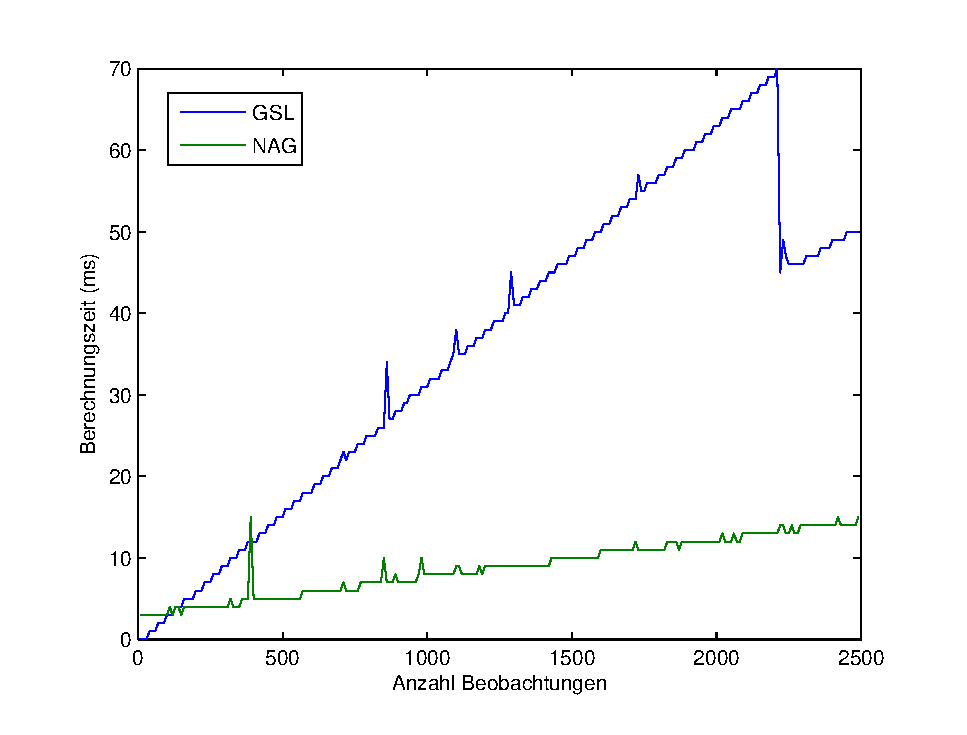
\includegraphics[width=9.5cm]{figures/simple_reg_comp_rent.eps}
  \end{figure}

\end{frame}

\begin{frame}
  \frametitle{Test einfache Regression II}

  \begin{itemize}
  \item Zufällige Daten:
  \end{itemize}
  
  \begin{figure}[t]
    \centering
    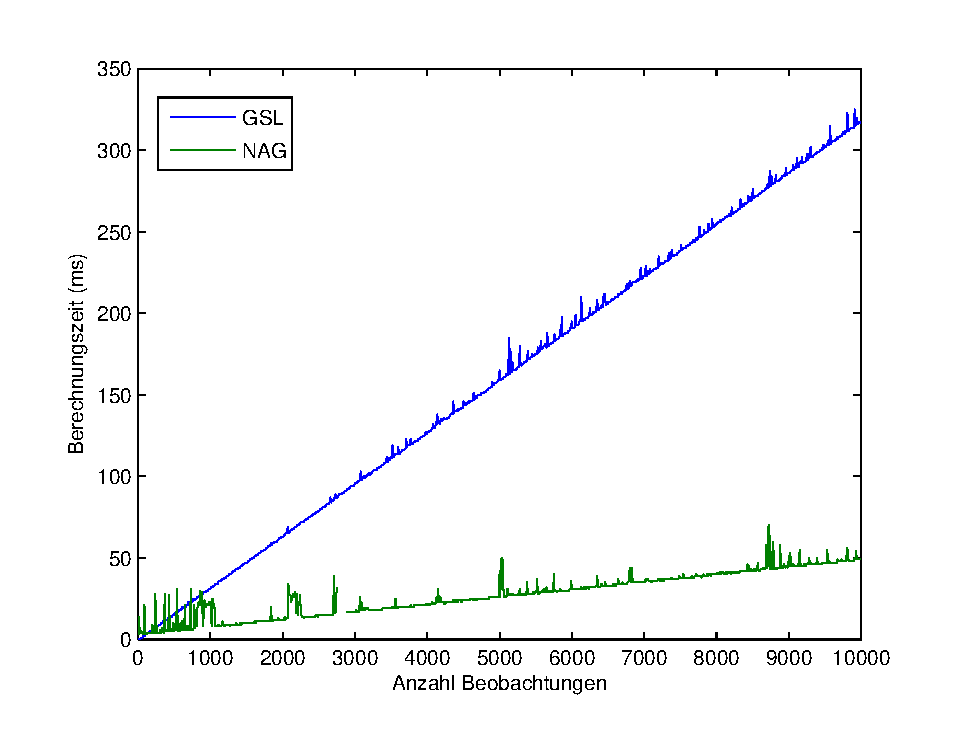
\includegraphics[width=9.5cm]{figures/simple_reg_comp.eps}
  \end{figure}

\end{frame}

\begin{frame}
  \frametitle{Vergleich multiple Regression}
  
  \begin{block}{nag\_regsn\_mult\_linear}
    \begin{itemize}
    \item Regressionskoeffizienten
    \item Quadratsumme der Residuen
    \item Standartfehler
    \item Kovarianzmatrix
    \item Residuen
    \item (Zwischenergebnisse)
    \end{itemize}
  \end{block}
  
  \begin{block}{gsl\_multifit\_linear}
    \begin{itemize}
    \item Regressionskoeffizienten
    \item Quadratsumme der Residuen
    \item Kovarianzmatrix
    \end{itemize}
  \end{block}

\end{frame}

\begin{frame}[fragile]
  \frametitle{Funktionsaufrufe multiple Regression}
  
  \begin{columns}
    \column{0.5\textwidth}
    \begin{block}{Testprogramm NAG}
      \begin{lstlisting}
timer.start();

for(int i=1; i<=iterations; i++){
  
  nag_regsn_mult_linear(mean, 
    y_size, x, tdx, m, sx, ip, 
    y, wt, &rss, &df, b, se,
    cov, res, h, q, tdq, &svd, 
    &rank, p, tol, com_ar, &fail);

}

timer.stop();
      \end{lstlisting}
    \end{block}
    \column{0.5\textwidth}
    \begin{block}{Testprogramm GSL}
      \begin{lstlisting}
timer.start();

for(int i=1; i<=iterations; i++){    
  
  gsl_multifit_linear(x, y, c, 
    cov, &chisq, wspace);
  
  for(int i=0; i<ip; i++){
    gsl_vector_set(se, i, 
      sqrt(gsl_matrix_get(cov, 
            i, i)));
  }
    
  gsl_multifit_linear_residuals(x, 
    y, c, r);
}

timer.stop();
\end{lstlisting}
\end{block}    
\end{columns}

\end{frame}

\begin{frame}
  \frametitle{Testaufbau multiple Regression}
  
  \begin{block}{Test 1:}
    \begin{itemize}
    \item Iterationen: 100
    \item Unabhängige Merkmale: 6
    \item Beobachtungen variabel
    \end{itemize}
  \end{block}

  \begin{block}{Test 2:}
    \begin{itemize}
    \item Iterationen: 100
    \item Beobachtungen: 2500
    \item Unabhängige Merkmale variabel
    \end{itemize}
  \end{block}
  
  \begin{itemize}
  \item Datensätze:
    \begin{itemize}
    \item Mietdatensatz
    \item Zufällig erzeugte Daten
    \end{itemize}
  \end{itemize}
  
\end{frame}

\begin{frame}
  \frametitle{Test multiple Regression}

  \begin{itemize}
  \item Zufällige Daten:
  \end{itemize}

  \begin{figure}[t]
    \centering
    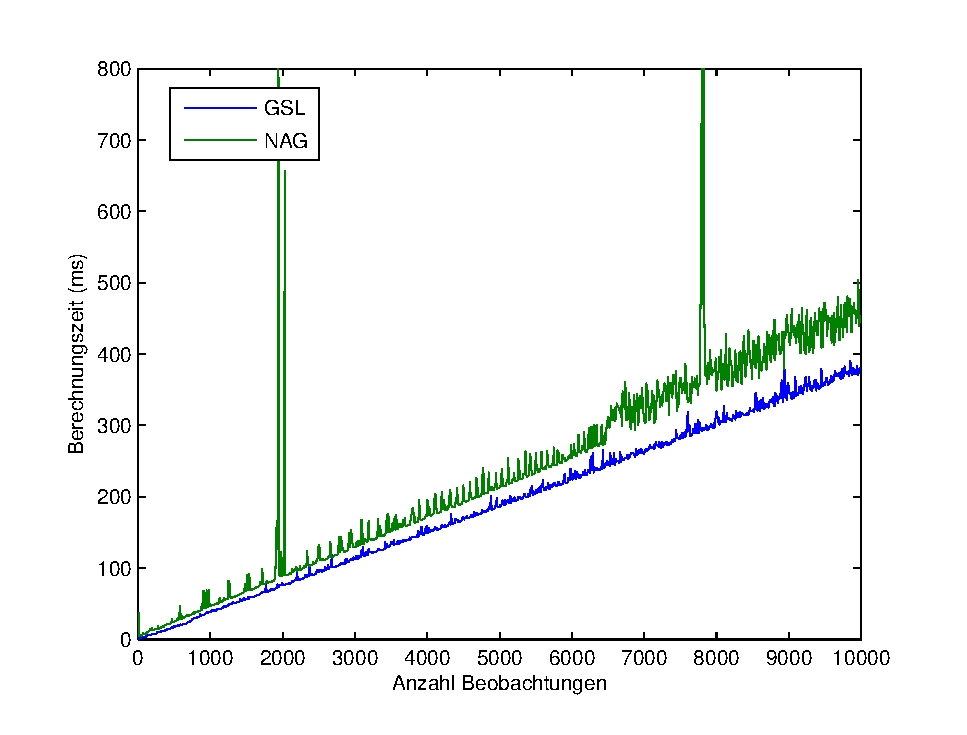
\includegraphics[width=9.5cm]{figures/multi_reg_comp_6_var.eps}
  \end{figure}

\end{frame}

\begin{frame}
  \frametitle{Test multiple Regression II}
  \begin{itemize}
  \item Mietdatensatz:
  \end{itemize}

  \begin{figure}[t]
    \centering
    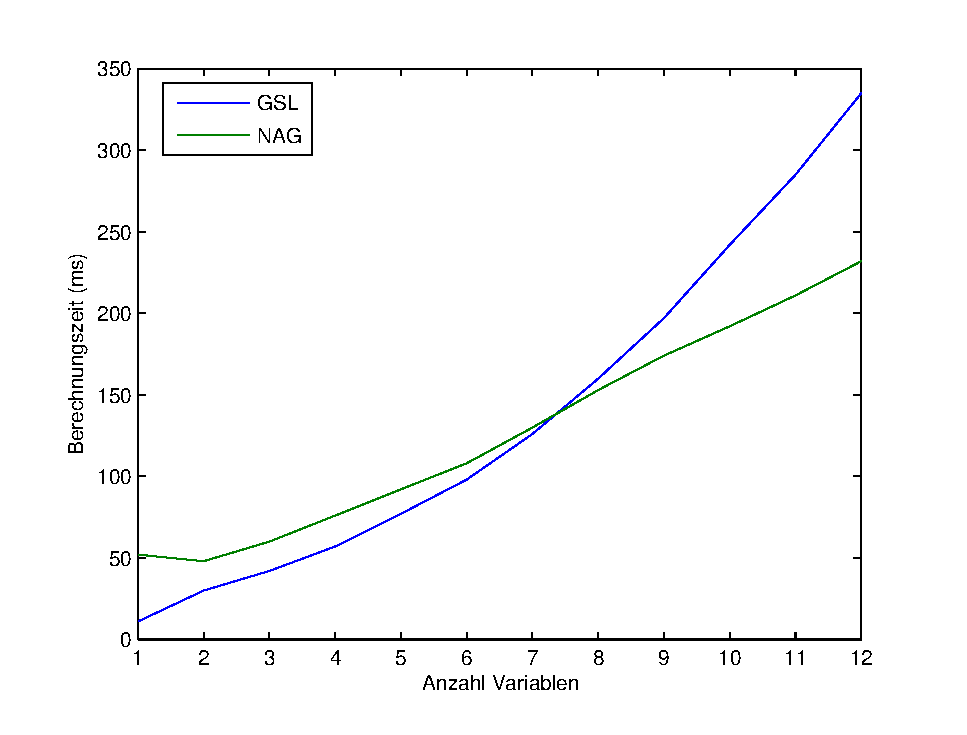
\includegraphics[width=9.5cm]{figures/multi_reg_vars_2500_obs.eps}
  \end{figure}
\end{frame}

\begin{frame}
  \frametitle{Test multiple Regression III}
  \begin{itemize}
  \item Zufällige Daten:
  \end{itemize}

  \begin{figure}[t]
    \centering
    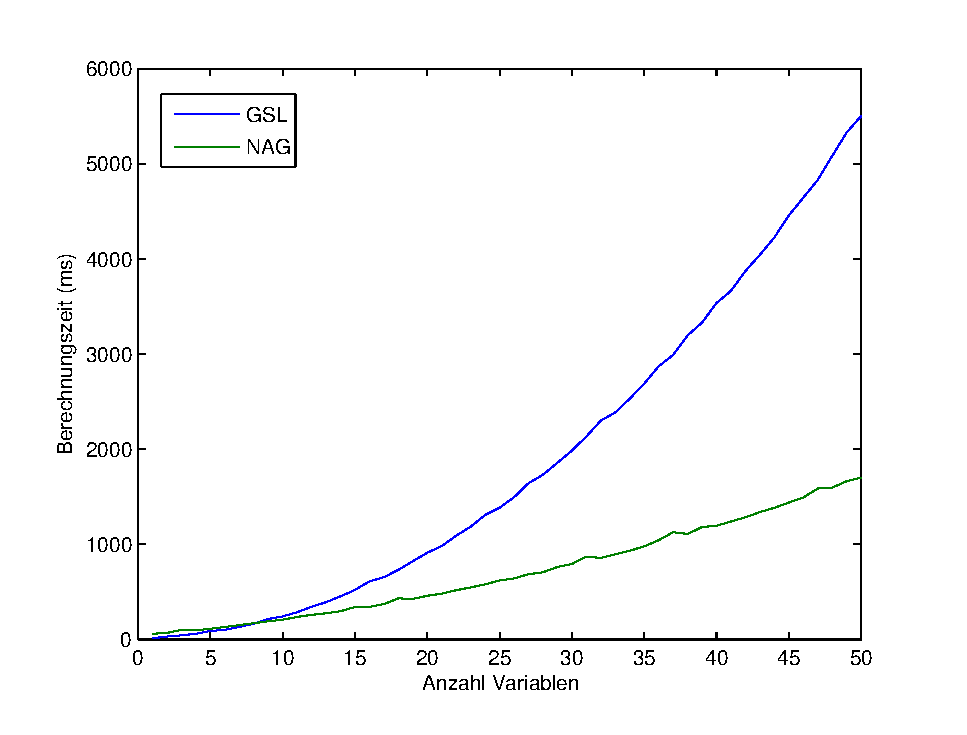
\includegraphics[width=9.5cm]{figures/multi_reg_vars_2500_obs_rand.eps}
  \end{figure}

\end{frame}

\begin{frame}
  \frametitle{Aktualisierung vs. Neuberechnung}
    
  \begin{itemize}
  \item Funktionen zum Aktualisieren des Modells:
    \begin{itemize}
    \item nag\_regsn\_mult\_linear\_addrem\_obs
    \item \alert<3>{nag\_regsn\_mult\_linear\_add\_var}
    \item nag\_regsn\_mult\_linear\_delete\_var
    \item nag\_regsn\_mult\_linear\_addrem\_obs
    \item \alert<3>{nag\_regsn\_mult\_linear\_update\_model}
    \end{itemize}
  \end{itemize}

  \pause

  \begin{itemize}
  \item Wie ändert sich die Performance mit diesen Funktionen?
  \end{itemize}

  \pause

  \begin{itemize}
  \item Testparameter:
    \begin{itemize}
    \item Iterationen: 100
    \item Bobachtungen 2500
    \end{itemize}
  \end{itemize}

\end{frame}

\begin{frame}
  \frametitle{Test Aktualisierung}
  
  \begin{itemize}
  \item Mietdatensatz:
  \end{itemize}

  \begin{figure}[t]
    \centering
    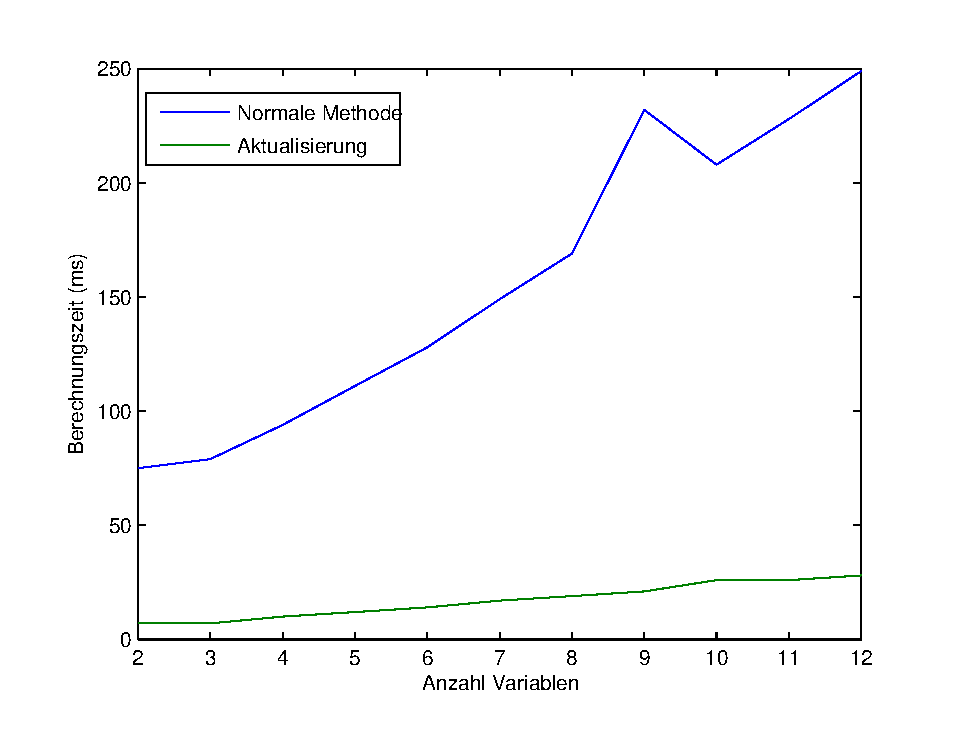
\includegraphics[width=9.5cm]{figures/multi_reg_vars_2500_obs_act.eps}
  \end{figure}

\end{frame}

\begin{frame}
  \frametitle{Test Aktualisierung II}
  
  \begin{itemize}
  \item Zufällige Daten:
  \end{itemize}

  \begin{figure}[t]
    \centering
    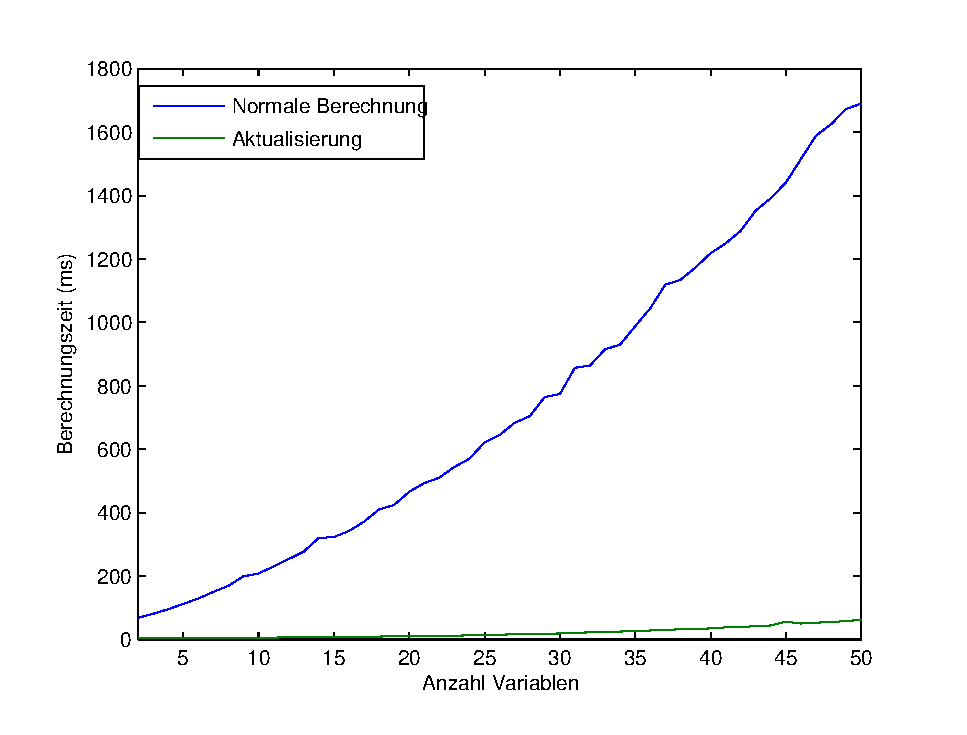
\includegraphics[width=9.5cm]{figures/multi_reg_vars_2500_obs_act_rand.eps}
  \end{figure}

\end{frame}


\section{Fazit}
\begin{frame}
  \frametitle{Fazit}
  
  \begin{itemize}
  \item NAG Bibliothek für Korrelation und Regression gut geeignet
  \item Im Vergleich zur GSL:
    \begin{itemize}
    \item (Meist) effizientere Implementierung
    \item Größerer Funktionsumfang
    \item Zusätzliche Hilfsfunktionen (z.B. nag\_step\_regsn)
    \item Funktionen werden umfangreich getestet
    \end{itemize}
  \end{itemize}
  
\end{frame}

\begin{frame}
  \frametitle{}

  \begin{center}
    {\Large Vielen Dank für die Aufmerksamkeit!}
  \end{center}

\end{frame}

\end{document}
